\documentclass[12pt]{article}

% packages
\usepackage[margin=1in]{geometry}
\usepackage[labelfont=it, justification=centering]{caption}
\usepackage{subcaption}
\usepackage{framed}
\usepackage[table]{xcolor}
\usepackage{colortbl, multirow}
\usepackage{amsmath,amsthm,amssymb,wasysym}
\usepackage{mathrsfs, mathtools}
\usepackage{tikz,pgf,pgfplots}
\usetikzlibrary{arrows, angles, quotes, decorations.pathreplacing, math, patterns, calc}
\usepackage{graphicx}

% custom commands
\newcommand{\N}{\mathbb{N}}
\newcommand{\Z}{\mathbb{Z}}
\newcommand{\I}{\mathbb{I}}
\newcommand{\R}{\mathbb{R}}
\newcommand{\Q}{\mathbb{Q}}
\newcommand{\p}{^{\prime}}
\newcommand{\powerset}{\raisebox{.15\baselineskip}{\Large\ensuremath{\wp}}}
\DeclarePairedDelimiter{\ceil}{\lceil}{\rceil}
\DeclarePairedDelimiter\floor{\lfloor}{\rfloor}

 
\begin{document}
 
\title{Assignment 1\\
    \large MATH CS 120FG Graph Theory I}
\author{Harry Coleman}
\date{January 16, 2020}

\maketitle

\section*{Exercise 1}
\fbox{
    \parbox{\textwidth} {
        Find three mutually non-isomorphic graphs each with degree sequence (5, 3, 2, 2, 1, 1, 1, 1).
    }
}
\\

\begin{figure}[ht]
    \centering
    \begin{subfigure}[b]{.3\textwidth}
        \centering
        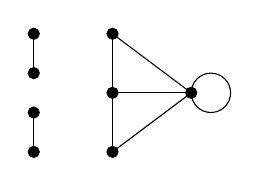
\begin{tikzpicture}
            \foreach \x\y in {0/0, 0/0.5, 0/1, 0/1.5, 1/0, 1/0.75, 1/1.5, 2/0.75} {
                \draw[fill=black] (\x,\y) circle (2pt);
            }
            
            \draw[] (0,0)--(0,0.5) (0,1)--(0,1.5);
            \draw[] (1,.75)--(2,0.75);
            \draw[] (1,0)--(1,1.5);
            \draw[] (1,0)--(2,0.75) (1,1.5)--(2,0.75);
            
            \draw[] (2.25,0.75) circle (0.25);
        \end{tikzpicture}
        \caption{}
        \label{fig:ex1-1}
    \end{subfigure}
    \begin{subfigure}[b]{.3\textwidth}
        \centering
        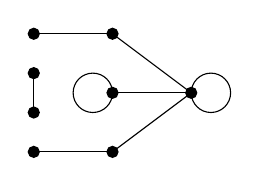
\begin{tikzpicture}
            \foreach \x\y in {0/0, 0/0.5, 0/1, 0/1.5, 1/0, 1/0.75, 1/1.5, 2/0.75} {
                \draw[fill=black] (\x,\y) circle (2pt);
            }
            
            \draw[] (0,0)--(1,0) (0,1.5)--(1,1.5);
            \draw[] (0,0.5)--(0,1);
            \draw[] (1,.75)--(2,0.75);
            \draw[] (1,0)--(2,0.75) (1,1.5)--(2,0.75);
            
            \draw[] (2.25,0.75) circle (0.25);
            \draw[] (0.75,0.75) circle (0.25);
        \end{tikzpicture}
        \caption{}
        \label{fig:ex1-2}
    \end{subfigure}
    \begin{subfigure}[b]{.3\textwidth}
        \centering
        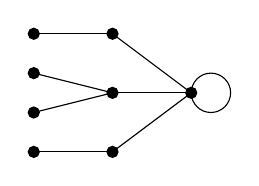
\begin{tikzpicture}
            \foreach \x\y in {0/0, 0/0.5, 0/1, 0/1.5, 1/0, 1/0.75, 1/1.5, 2/0.75} {
                \draw[fill=black] (\x,\y) circle (2pt);
            }
            
            \draw[] (0,0)--(1,0) (0,1.5)--(1,1.5);
            \draw[] (0,0.5)--(1,0.75)--(0,1);
            \draw[] (1,.75)--(2,0.75);
            \draw[] (1,0)--(2,0.75) (1,1.5)--(2,0.75);
            
            \draw[] (2.25,0.75) circle (0.25);
        \end{tikzpicture}
        \caption{}
        \label{fig:ex1-3}
    \end{subfigure}
    \caption{}
    \label{fig:ex1}
\end{figure}


\section*{Exercise 2}
\fbox{
    \parbox{\textwidth} {
        Let $(d_1, d_2, . . . , d_n)$ be any non-increasing sequence of nonnegative integers. Show that if $\Sigma_i d_i$ is even, then there exists a graph with this degree sequence (possibly with loops or parallel edges!).
    }
}
\\

We will consider each $d_i$ to uniquely represent the "desired" degree of a vertex in our graph. We imagine drawing and labeling all the points. At this moment, every vertex has a degree of zero.

Since the sum of all of the desired degrees of all the vertices is even, there must be an even number of vertices with odd desired degree. This means we can uniquely pair each vertex of odd desired degree with another such vertex. In each of these pairs, we create an edge connecting the two vertices. Now each vertex with an odd desired degree currently has degree 1. 

Now, for each vertex, the difference between its current degree and its desired degree is some even number. To each vertex, we add half this number of loops, so its current degree becomes its desired degree. After this, we have created a graph with the given degree sequence.


\newpage
\section*{Exercise 5}
\fbox{
    \parbox{\textwidth} {
        Suppose that $P$ and $Q$ are two maximum length paths in a connected graph $G$. Prove that $P$ and $Q$ have a common vertex.
    }
}
\\

Let $n$ be the length of both $P$ and $Q$. To show $P$ and $Q$ have a common vertex, we assume the opposite is true: that $P$ and $Q$ have no common vertex. Since $P$ and $Q$ are part of a connected graph, there must be a path from some vertex in $P$ to some vertex in $Q$. In other words, if we let
\begin{align*}
    P &= (p_1, p_2, \dots, p_i, \dots, p_n), \\
    Q &= (q_1, q_2, \dots, q_j, \dots, q_n),
\end{align*}
then for some $p_i, q_j$, there exists a path in $G$ from $p_i$ to $q_j$. If this path contains another vertex in $P$, we simply take the portion of the path from that vertex, likewise if the path contains another vertex in $Q$. We let $p_i$ and $q_j$ be the ends of a path in $G$ which contains no other points in $P$ or $Q$.

Without loss of generality, we assume $i\geq j$. The path
\[(p_1, \dots, p_i, \dots, q_j, \dots, q_n)\]
has length
\[i + k + (n-j+1) > n \]
where $k$ is the number of vertices in the path from $p_i$ to $q_j$ that are not $p_i$ or $q_j$. So there is a path in $G$ which is longer than both $P$ and $Q$, therefore neither $P$ nor $Q$ are maximum length paths. This is a contradiction, so $P$ and $Q$ must have some common vertex.


\section*{Exercise 6}
\fbox{
    \parbox{\textwidth} {
        Suppose $W$ is a closed walk in $G$ and edge $e \in E(G)$ appears an odd number of times in $W$. Prove that $W$ contains a cycle using $e$.
    }
}
\\

Let $u,v$ be the vertices of such that $e=(u,v)$. To show that there is a cycle in $W$ using $e$, we must show that there is a walk in $W$, and therefore path, from $v$ to $u$ which does not use $e$. A path in $W$ from $v$ to $u$ without $e$ then from $u$ to $v$ using $e$ would be a cycle in $W$.

To show there is a walk from $v$ to $u$ in $W$, we will assume there is no such walk. We now consider tracing $W$, starting at $u$. Since there is no walk in $W$ from $u$ to $v$ which does not use $e$, the first time $e$ appears in $W$, it is from $u$ to $v$. The second time $e$ appears, it is from $v$ to $u$, and so on. For every $n$th occurrence of $e$: if $n$ is odd we go from $u$ to $v$, if $n$ is even we go from $v$ to $u$. Since $e$ occurs an odd number of times in $W$, the last time $e$ is used, it is from $u$ to $v$.

However, since we supposed no walk from $v$ to $u$ without $e$ exists in $W$, and we started at $u$, $W$ cannot be a closed walk. This is a contradiction, so a walk, and therefore a path, from $v$ to $u$ without $e$ exists in $W$. Taking this path, with $e$, gives a cycle in $W$ which uses $e$.


\newpage
\section*{Exercise 7}
\fbox{
    \parbox{\textwidth} {
        For $n \geq 1$, let $R_n$ be the graph with vertex set ${0, 1}^n$ (i.e., binary n-tuples), but with two vertices adjacent if they differ in exactly two positions. Determine the number of components in $R_n$.
    }
}
\\

Let $x$ and $y$ be two vertices of $R_n$. We define $x_i$ (respectively $y_i$) to be the $i$th value in the binary sequence related to $x$ (respectively $y$). In $R_n$, two vertices are adjacent if and only if their related binary sequences differ in exactly two places.

Suppose $x$ and $y$ are adjacent, this tells us that for some $k,l$, we know $x_i=y_i$ if and only if $i$ is not $k$ or $l$. With all other values in $x$ and $y$ the same, we have the following:
\begin{align*}
    x_k = 0, x_l = 0 &\iff y_k=1, y_l=1, \\
    x_k = 0, x_l = 1 &\iff y_k=1, y_l=0, \\
    x_k = 1, x_l = 0 &\iff y_k=0, y_l=1, \\
    x_k = 1, x_l = 1 &\iff y_k=0, y_l=0. \\
\end{align*}

In all of these cases, the amount of "1"s in $x$ and $y$ are either the same, or differ by 2. This means that $x\sim y$ if and only if the amount of "1"s in their related binary sequences differ by 0 or 2. This means that a walk from $x$ to $y$ in $R_n$ exists if and only if the amount of "1"s in their related binary sequences differ by a multiple of 2 (both even or odd).

This means $R_n$ has two components: one where all vertices have related binary sequences with an even amount of "1"s, and another for an odd amount of "1"s.


\section*{Exercise 8}
\fbox{
    \parbox{\textwidth} {
        Show that if $G$ is self-complementary, then the number of vertices of $G$ is congruent to either 0 or 1 modulo 4. Moreover, construct a self-complementary graph for any $n \equiv 0, 1 \pmod{4}$.
    }
}
\\

Suppose we have a graph $G$ that is self-complementary. This means that $G$ is isomorphic to it's complement $\overline{G}$. If $G$ has $n$ vertices, then there are
\[{n \choose 2} = \frac{n(n-1)}{2}\]
possible edges between those vertices. Since each possible edge shows up in either $G$ or $\overline{G}$, but not both. Since $G$ and $\overline{G}$ must have the same number of edges, then each has exactly
\[\frac{n(n-1)}{4}\]
edges. So $n(n-1)$ must be equivalent to 0 modulo 4. We consider the possible cases for $n$ modulo 4:
\begin{align*}
    n &\equiv 0 & n(n-1)\equiv 0(3) & \equiv 0 \pmod{4} \\
    n &\equiv 1 & n(n-1)\equiv 1(0) & \equiv 0 \pmod{4} \\
    n &\equiv 2 & n(n-1)\equiv 2(1) & \equiv 2 \pmod{4} \\
    n &\equiv 3 & n(n-1)\equiv 3(2) & \equiv 2 \pmod{4}
\end{align*}
So $n$, which is the number of vertices in $G$, must be equivalent to 0 or 1 modulo 4.

In order to construct the self complementary graph with $n$ vertices for an arbitrary $n \equiv 0, 1 \pmod{4}$, we first consider the the base case of $n=4$, shown in figure \ref{fig:n4}.

\begin{figure}[ht]
    \centering
    \begin{subfigure}[b]{.3\textwidth}
        \centering
        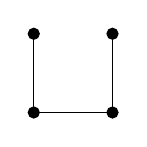
\begin{tikzpicture}
            \foreach \x\y in {0/0, 0/1, 1/0, 1/1} {
                \draw[fill=black] (\x,\y) circle (2pt);
            }
            
            \draw[] (0,0)--(1,0);
            \draw[] (0,0)--(0,1);
            \draw[] (1,0)--(1,1);
            
        
        \end{tikzpicture}
        \caption{}
        \label{fig:n4a}
    \end{subfigure}
    \begin{subfigure}[b]{.3\textwidth}
        \centering
        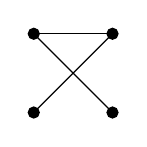
\begin{tikzpicture}
            \foreach \x\y in {0/0, 0/1, 1/0, 1/1} {
                \draw[fill=black] (\x,\y) circle (2pt);
            }
            
            \draw[] (0,1)--(1,1);
            \draw[] (0,1)--(1,0);
            \draw[] (1,1)--(0,0);
        \end{tikzpicture}
        \caption{}
        \label{fig:n4b}
    \end{subfigure}
    \caption{Self-Complementary Graph with $n=4$.}
    \label{fig:n4}
\end{figure}

For each $n=4k$, with $k\in\N$, we simply place a cluster of $k$ vertices where we see a single vertex in $n=4$. Where we see an edge in $n=4$, we create an edge between each vertex of one cluster and each vertex of the opposite cluster. In other words, we create a complete bipartite subgraph between the two clusters. For the clusters corresponding to the bottom two vertices in figure \ref{fig:n4a}, we connect each two vertices in the same clusters. In other words, the bottom two clusters become two cliques, whereas the top two clusters stay independent sets.

When we take the complement of this graph, we obtain the same overall structure as that in figure \ref{fig:n4b}. The top two clusters become cliques, the bottom two clusters become independent sets, and each top cluster is half of a complete bipartite subraph with each other and one bottom cluster. The graph for $n=12$ is given in figure \ref{fig:n12}.

\begin{figure}[ht]
    \centering
    \begin{subfigure}[b]{.3\textwidth}
        \centering
        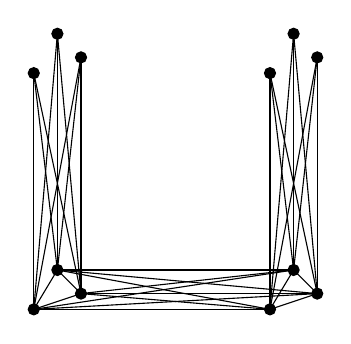
\begin{tikzpicture}
            \foreach \x\y in {0/0, 0/3, 3/0, 3/3} {
                \draw[fill=black] (\x,\y) circle (2pt);
                \draw[fill=black] (\x-0.3,\y-0.5) circle (2pt);
                \draw[fill=black] (\x+0.3,\y-0.3) circle (2pt);
            }
            
            \foreach \xi\yi\xj\yj in {0/0/0/3, 3/0/3/3, 0/0/3/0} {
                \foreach \ai\bi in {0/0, 0.3/-0.3, -0.3/-0.5} {
                    \foreach \aj\bj in {0/0, 0.3/-0.3, -0.3/-0.5} {
                        \draw[] (\xi+\ai, \yi+\bi)--(\xj+\aj, \yj+\bj);
                    }
                }
            }
            
            \foreach \x\y in {0/0, 3/0} {
                \draw[] (\x, \y)--(\x+0.3, \y-0.3);
                \draw[] (\x, \y)--(\x-0.3, \y-0.5);
                \draw[] (\x-0.3, \y-0.5)--(\x+0.3, \y-0.3);
            }
        \end{tikzpicture}
        \caption{}
        \label{fig:n12a}
    \end{subfigure}
    \begin{subfigure}[b]{.3\textwidth}
        \centering
        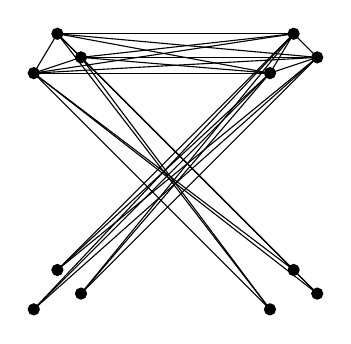
\begin{tikzpicture}
            \foreach \x\y in {0/0, 0/3, 3/0, 3/3} {
                \draw[fill=black] (\x,\y) circle (2pt);
                \draw[fill=black] (\x-0.3,\y-0.5) circle (2pt);
                \draw[fill=black] (\x+0.3,\y-0.3) circle (2pt);
            }
            
            \foreach \xi\yi\xj\yj in {0/0/3/3, 3/0/0/3, 0/3/3/3} {
                \foreach \ai\bi in {0/0, 0.3/-0.3, -0.3/-0.5} {
                    \foreach \aj\bj in {0/0, 0.3/-0.3, -0.3/-0.5} {
                        \draw[] (\xi+\ai, \yi+\bi)--(\xj+\aj, \yj+\bj);
                    }
                }
            }
            
            \foreach \x\y in {0/3, 3/3} {
                \draw[] (\x, \y)--(\x+0.3, \y-0.3);
                \draw[] (\x, \y)--(\x-0.3, \y-0.5);
                \draw[] (\x-0.3, \y-0.5)--(\x+0.3, \y-0.3);
            }
        \end{tikzpicture}
        \caption{}
        \label{fig:n12b}
    \end{subfigure}
    \caption{Self-Complementary Graph with $n=3k=12$.}
    \label{fig:n12}
\end{figure}

For graphs with $n=4k+1$, we simply add an additional vertex which is connected to all vertices in the bottom two clusters. When we take the complement, this will be connected to all the vertices in the top two clusters.






\end{document}